% id: 88-68
% book: 쎈B 미적분1 · 06 도함수의 활용 (3)
% section: 유형 17 시각에 대한 길이의 변화율
% figure: crop:fig-88-68.jpg
% answer: 
% answer_source: 
% variant_level: 0 (원본 전사)
% 이 파일은 build.mjs 가 items.json 에서 만든다. 고칠 때는 items.json 을 고친다.
\smash{\raisebox{1.5mm}{\dmkichul{쎈B 미적분1 88쪽 68번 · 대표 문제}}}
\noindent\begin{minipage}[t]{0.58\linewidth}\vspace{0pt}\raggedright 오른쪽 그림과 같이 키가 $1.6\mkern3mu \mathrm{m}$인 사람이 높이 $4\mkern3mu \mathrm{m}$의 가로등 바로 밑에서 출발하여 매초 $1.5\mkern3mu \mathrm{m}$의 속도로 일직선으로 걸어가고 있다. 이때 이 사람의 그림자의 길이의 변화율은?\end{minipage}\hfill\begin{minipage}[t]{0.4\linewidth}\vspace{0pt}\centering 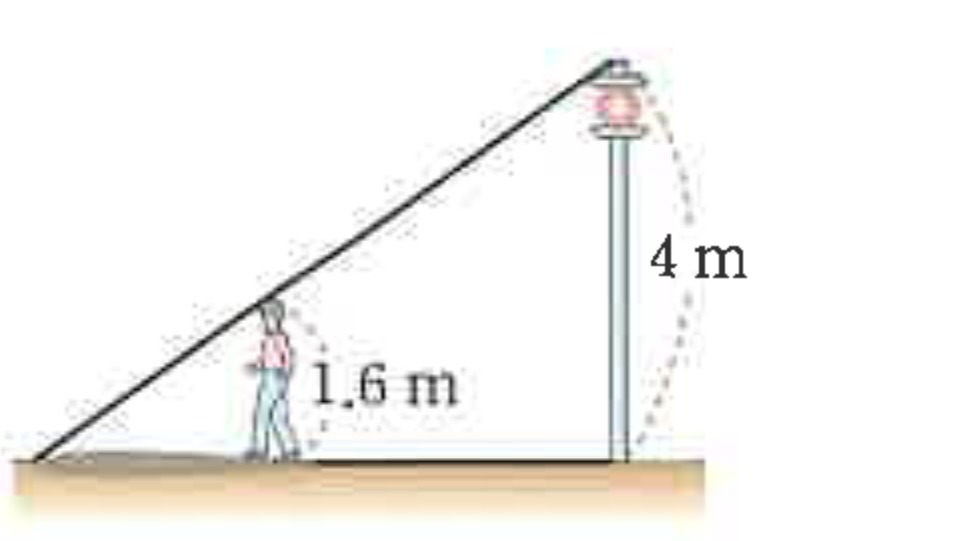
\includegraphics[width=0.92\linewidth]{figures/fig-88-68.jpg}\end{minipage}\par
\begin{choices32}{$1\mkern3mu \mathrm{m/s}$}{$1.2\mkern3mu \mathrm{m/s}$}{$1.5\mkern3mu \mathrm{m/s}$}{$1.8\mkern3mu \mathrm{m/s}$}{$2\mkern3mu \mathrm{m/s}$}\end{choices32}
